%%
%% This is file `sample-xelatex.tex',
%% generated with the docstrip utility.
%%
%% The original source files were:
%%
%% samples.dtx  (with options: `sigconf')
%% 
%% IMPORTANT NOTICE:
%% 
%% For the copyright see the source file.
%% 
%% Any modified versions of this file must be renamed
%% with new filenames distinct from sample-xelatex.tex.
%% 
%% For distribution of the original source see the terms
%% for copying and modification in the file samples.dtx.
%% 
%% This generated file may be distributed as long as the
%% original source files, as listed above, are part of the
%% same distribution. (The sources need not necessarily be
%% in the same archive or directory.)
%%
%% The first command in your LaTeX source must be the \documentclass command.
\documentclass[sigchi]{acmart}

\usepackage{graphicx}
\usepackage{textgreek}
\usepackage{xcolor}
\usepackage{tabularx}
\usepackage{makecell}
% \usepackage[utf8]{inputenc}
% \usepackage[T1]{fontenc}


%%
%% \BibTeX command to typeset BibTeX logo in the docs
\AtBeginDocument{%
  \providecommand\BibTeX{{%
    \normalfont B\kern-0.5em{\scshape i\kern-0.25em b}\kern-0.8em\TeX}}}

\settopmatter{printacmref=false}
\settopmatter{printfolios=true}

%% Rights management information.  This information is sent to you
%% when you complete the rights form.  These commands have SAMPLE
%% values in them; it is your responsibility as an author to replace
%% the commands and values with those provided to you when you
%% complete the rights form.
\setcopyright{iw3c2w3g}
\copyrightyear{}
\acmYear{}
\acmDOI{}

%% These commands are for a PROCEEDINGS abstract or paper.
\acmConference[]{}{}{}
\acmBooktitle{}
\acmPrice{}
\acmISBN{}


%%
%% Submission ID.
%% Use this when submitting an article to a sponsored event. You'll
%% receive a unique submission ID from the organizers
%% of the event, and this ID should be used as the parameter to this command.
%%\acmSubmissionID{123-A56-BU3}

%%
%% The majority of ACM publications use numbered citations and
%% references.  The command \citestyle{authoryear} switches to the
%% "author year" style.
%%
%% If you are preparing content for an event
%% sponsored by ACM SIGGRAPH, you must use the "author year" style of
%% citations and references.
%% Uncommenting
%% the next command will enable that style.
%%\citestyle{acmauthoryear}

%%
%% end of the preamble, start of the body of the document source.
\begin{document}

%%
%% The "title" command has an optional parameter,
%% allowing the author to define a "short title" to be used in page headers.
\title{College Majors, Earnings, and Employability: A Visual Investigation}

%%
%% The "author" command and its associated commands are used to define
%% the authors and their affiliations.
%% Of note is the shared affiliation of the first two authors, and the
%% "authornote" and "authornotemark" commands
%% used to denote shared contribution to the research.
\author{David Kwan}
% \authornote{Both authors contributed equally to this research.}
\email{dkwan33@yorku.ca}
% \orcid{1234-5678-9012}
\affiliation{%
  \institution{York University}
  \streetaddress{4700 Keele St.}
  \city{Toronto}
  \state{Ontario}
  \postcode{M3J 1P3}
}

%%
%% By default, the full list of authors will be used in the page
%% headers. Often, this list is too long, and will overlap
%% other information printed in the page headers. This command allows
%% the author to define a more concise list
%% of authors' names for this purpose.
% \renewcommand{\shortauthors}{Trovato and Tobin, et al.}

%%
%% The abstract is a short summary of the work to be presented in the
%% article.
\begin{abstract}
  A clear and well-documented \LaTeX\ document is presented as an
  article formatted for publication by ACM in a conference proceedings
  or journal publication. Based on the ``acmart'' document class, this
  article presents and explains many of the common variations, as well
  as many of the formatting elements an author may use in the
  preparation of the documentation of their work.
\end{abstract}

%%
%% The code below is generated by the tool at http://dl.acm.org/ccs.cfm.
%% Please copy and paste the code instead of the example below.
%%
% \begin{CCSXML}
% <ccs2012>
%  <concept>
%   <concept_id>10010520.10010553.10010562</concept_id>
%   <concept_desc>Computer systems organization~Embedded systems</concept_desc>
%   <concept_significance>500</concept_significance>
%  </concept>
%  <concept>
%   <concept_id>10010520.10010575.10010755</concept_id>
%   <concept_desc>Computer systems organization~Redundancy</concept_desc>
%   <concept_significance>300</concept_significance>
%  </concept>
%  <concept>
%   <concept_id>10010520.10010553.10010554</concept_id>
%   <concept_desc>Computer systems organization~Robotics</concept_desc>
%   <concept_significance>100</concept_significance>
%  </concept>
%  <concept>
%   <concept_id>10003033.10003083.10003095</concept_id>
%   <concept_desc>Networks~Network reliability</concept_desc>
%   <concept_significance>100</concept_significance>
%  </concept>
% </ccs2012>
% \end{CCSXML}

% \ccsdesc[500]{Computer systems organization~Embedded systems}
% \ccsdesc[300]{Computer systems organization~Redundancy}
% \ccsdesc{Computer systems organization~Robotics}
% \ccsdesc[100]{Networks~Network reliability}

%%
%% Keywords. The author(s) should pick words that accurately describe
%% the work being presented. Separate the keywords with commas.
% \keywords{data sets, neural networks, gaze detection, text tagging}

%% A "teaser" image appears between the author and affiliation
%% information and the body of the document, and typically spans the
%% page.
% \begin{teaserfigure}
%   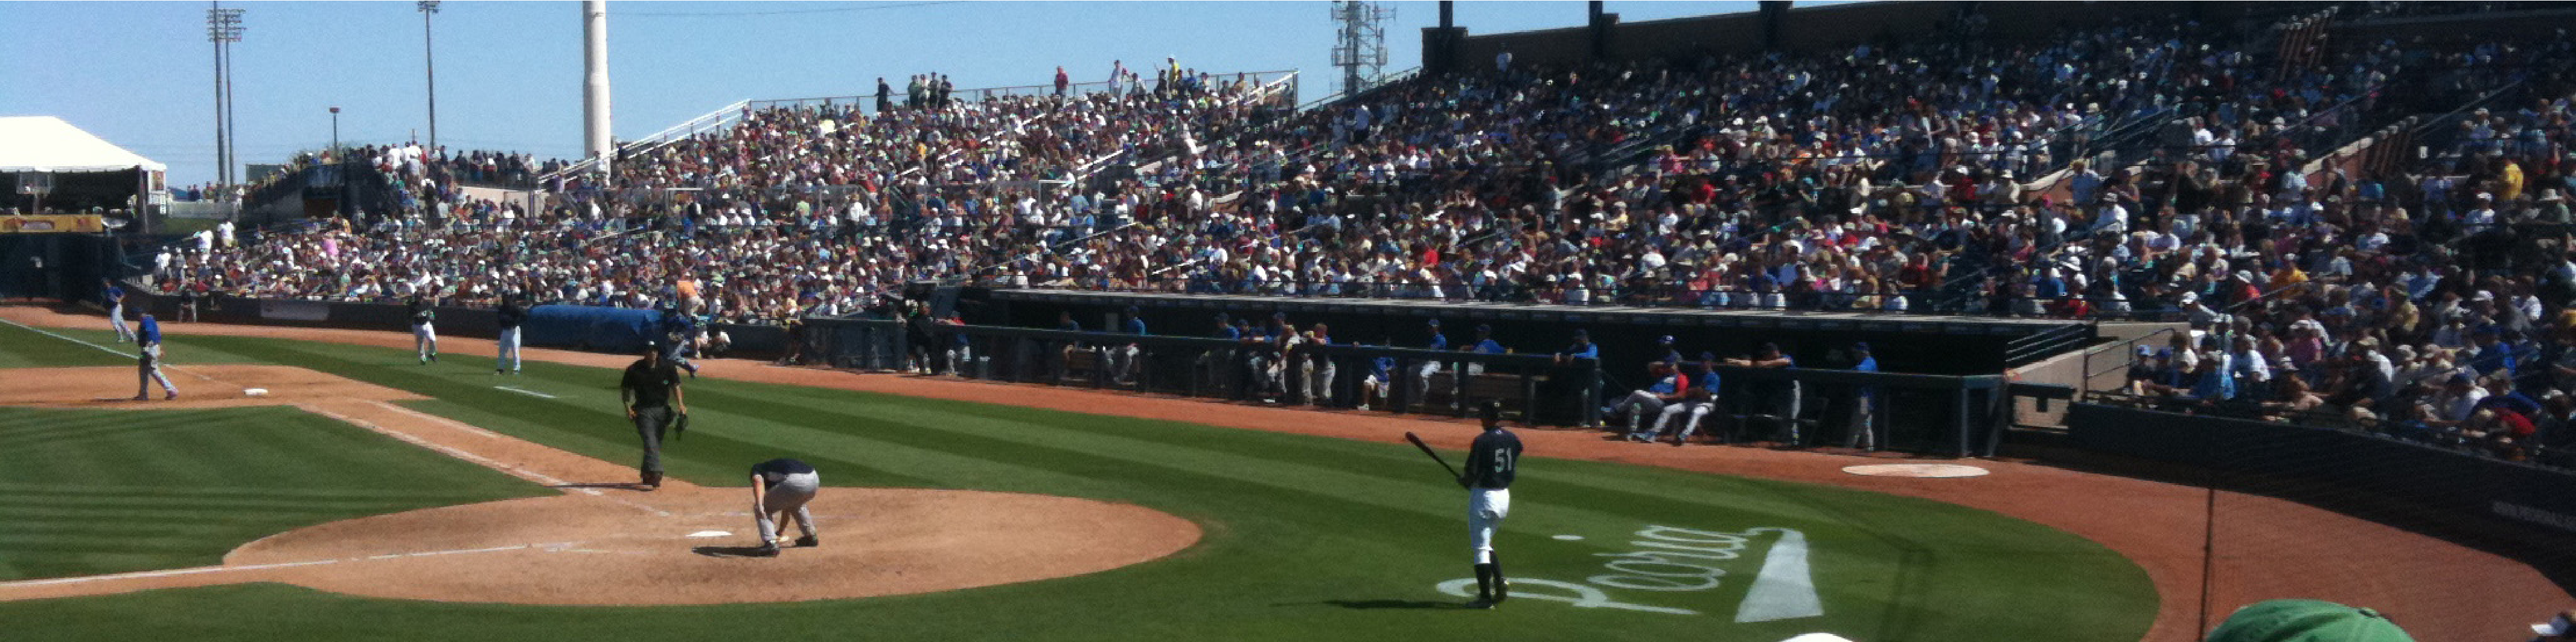
\includegraphics[width=\textwidth]{sampleteaser}
%   \caption{Seattle Mariners at Spring Training, 2010.}
%   \Description{Enjoying the baseball game from the third-base
%   seats. Ichiro Suzuki preparing to bat.}
%   \label{fig:teaser}
% \end{teaserfigure}

%%
%% This command processes the author and affiliation and title
%% information and builds the first part of the formatted document.
\maketitle

\section{Introduction}

For many students, perhaps almost every student, a major concern after graduation is employment. A college degree is by no means a guarantee of employment, nor is it a guarantee of economic safety, but it most certainly can help. The choice of major is a one of earliest decisions in a student's career, it can open many doors and offer many opportunities, but to many, the "wrong" choice may seem like a waste of time. After all, an unemployable or "useless" degree still takes just as much time as other degrees. There are a plethora of questions that prospective students, current students, or even recent graduates could be interested in: 
\begin{itemize}
\item{What kind of jobs are there?}
\item{What subjects are more popular?}
\item{What are students studying?}
\item{What do students specialize in?}
\item{Who makes more money?}
\item{Who is more employable?}
\item{Does the degree even matter?}
\end{itemize}
These are all valuable questions and are only a fraction of the possible questions regarding choice of college major. To that end, this investigation aims to answer all of the above and more using data visualization techniques with the Tableau software platform.

\section{Data Set}

In 2014, Ben Casselman wrote an article entitled \textit{The Economic Guide To Picking A College Major} published on the political and economic blog \textit{FiveThirtyEight} associated with ABC News \cite{fivethirtyeight}. This article used a full data set from the 2014 United States Census courtesy of the United States Census Bureau Public-Use Microdata. However, using this data set, Casselman only "ranked" the college majors in terms of earnings. Furthermore, Casselman did not create any data visualization. This is unfortunate as the data set itself holds much more potential. \textit{FiveThirtyEight} has made this data set public on Github (although the source was public to begin with, it is difficult to work with), along with the R script used to pull all the relevant data from the Census Bureau \cite{github}. 

The data itself is comprised of a few tables. The two most detailed contain data for recent graduates, being those of age 28 or less, as well as data pertaining to all ages. Each row pertains to a college major (e.g. Biomedical Engineering), and the first and foremost data column contains the broader major category (e.g. Engineering). Both of these are categorical data fields. The rest of the columns, of which there are many, are all quantitative. These data fields include the total number of people with that major, the total employed, the total unemployed, median salary of that major, gender, and much more. Data transformation was performed when required.

\section{Visualization Overview}

Using this data set, I have created a series of charts and dashboards using the Tableau platform. My focus is on recent graduates, so much of the data is from the recent graduates table, although data from the all-ages table are used as well whenever the comparison is worthwhile. 

The charts created include bar charts, box plots, scatterplots, and a map chart. Both the expressiveness and effectiveness principles of visualization design \cite{munzner} were adhered to as best as possible. Other available options such as packed-bubble charts were not chosen because it provided no clear advantage, even when placed on a dashboard with other types of charts. The map chart is a good example of a chart that, although does not strictly follow the expressiveness principle, had value especially when placed on a dashboard with interactivity.

Multiple dashboards were created with the goal of answering one or more specific questions that the user may have. All these dashboards provide value with interactive features, allowing the user to choose what they want to focus on. The interactivity cannot be shown here, nor is it particularly valuable to show screenshots of individual filters, but both filtering and highlighting can be done based on either major category or major specialization in all dashboards. This was immensely important for this data set considering that there were 172 different majors to choose from. It is reasonable to expect that most users would only be interested in a few, or even one major specialization, and the corresponding major field, and thus would want to highlight or filter for the major that they wanted to investigate.

Furthermore, the dashboards provide a juxtaposition between related graphs for comparison. One of the primary uses of juxtaposition in this case was to show a comparison between recent graduates and all ages along the same metrics. 

To avoid confusion in this paper, outside of the charts, "major" will be commonly referred to as "specialization", while "major category" will be commonly referred to as "field".

\section{Charts, Dashboards, Questions, and Answers}
\subsection{Dashboard 1: Fields and their Popularity}
\label{sec:db1}

  \begin{figure*}[thpb]
  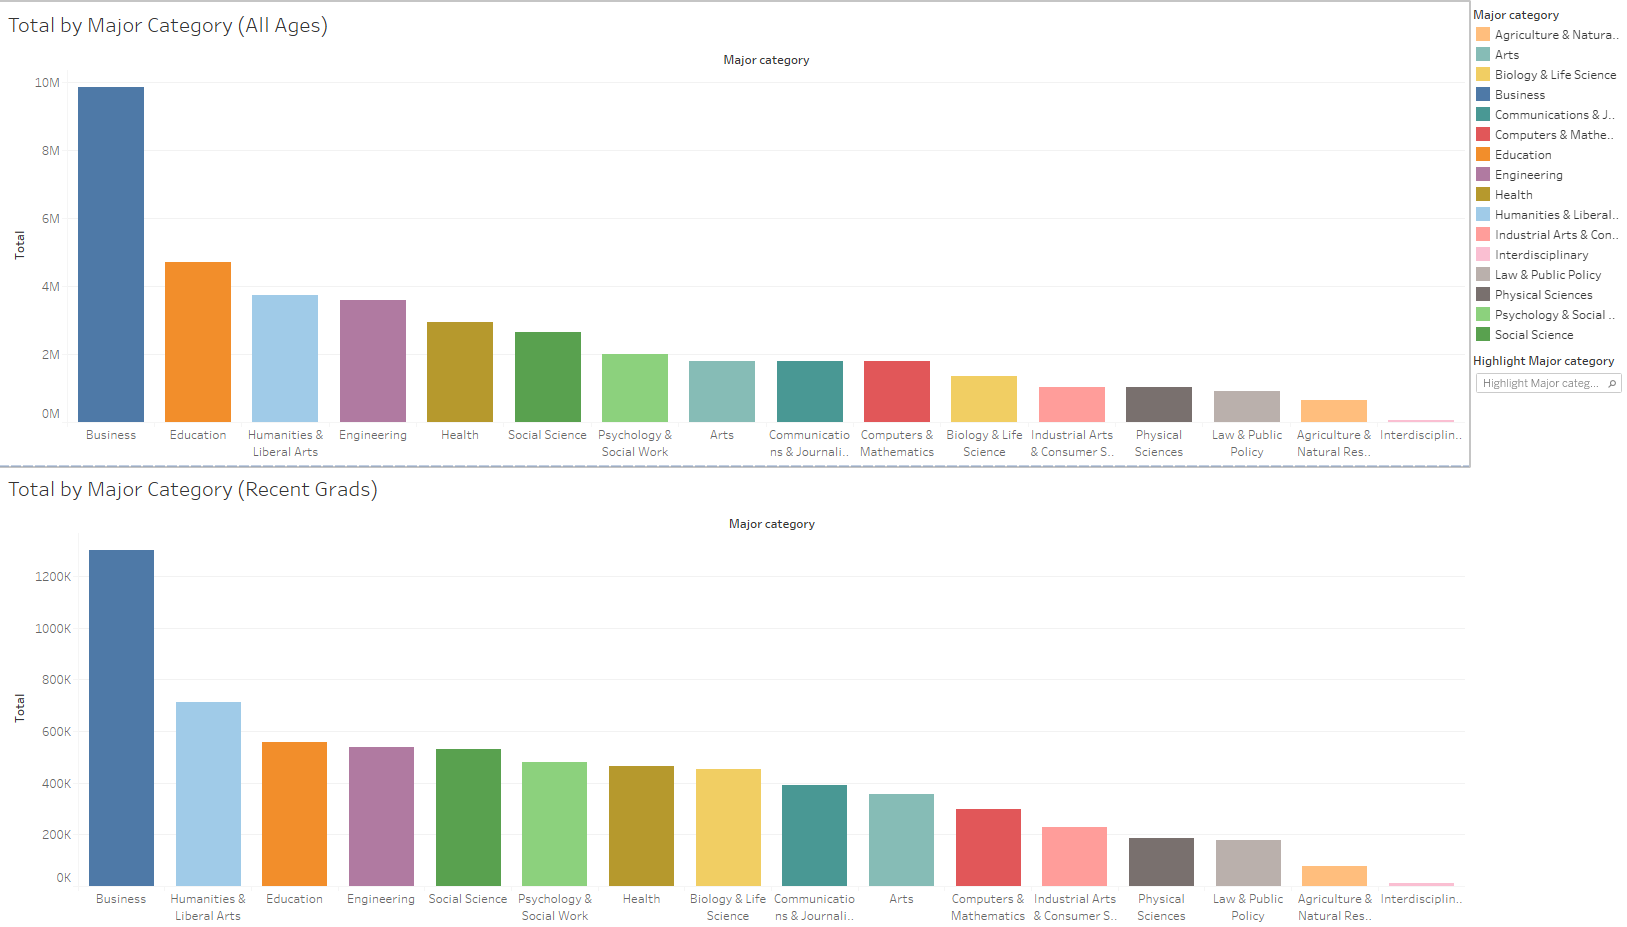
\includegraphics[width=1.0\textwidth]{DB1.png}
     \caption{Dashboard 1: Total Counts for each Major Category for both recent grads and all ages}
         \label{fig:db1}
  \end{figure*}
  
Dashboard 1 shown in Fig. \ref{fig:db1} attempts to introduce the user to the data set, as it only shows the major categories and not the major specializations. Following the expressiveness and effectiveness principles, the bar charts here represent the quantitative variable (Total) as height, while the categorical variable (Major category) is represented with colour hue. It is important to note here that the colours used for the major categories here are used throughout all the visualizations. This is important of course, for consistency. Furthermore, the large number of categories here means many colour hues had to be used, which after a certain point can confuse the reader and be hard to distinguish from one another. This is an unfortunate drawback to my visualization solution, but cannot be avoided, as the major categories cannot be further group, nor would it be fair to eliminate any as a base filter. 

This dashboard answers the question "What kind of jobs are there?". For now, we can assume what people are studying is representative of the jobs that exist, although section \ref{sec:db5} shows why this may not be the case when we look at under-utilization rate. It may be technically more accurate to say "What are people studying?" but that seems less pertinent to the intended reader. Clearly business is the dominant field in terms of popularity by a large margin. Physical sciences, Law, Agriculture are relatively unpopular. The juxtaposition of recent graduates vs all ages on this dashboard lets the reader infer if there are fields that are losing or gaining popularity. The most significant change seems to be a large increase in the current popularity of Biology \& Life Science.

\subsection{Dashboard 2: Specializations, Popularity, and an Introduction to Earnings}
\label{sec:db2}

\subsection{Dashboard 3: An In-Depth Look at Earnings}
\label{sec:db3}

** mention that salary is for all ages because there is much less of a difference for recent grads. it's all very similar
** Dashboard 2.5 did show bar graphs between salary of recent grads and not but was not useful as it was difficult to distinguish between differences in the heights even when juxtaposed. Furthermore, the difference in salary is pretty constant between all ages and recent grad for fields as a whole. Just a general increase with no significant outliers. Specific specialization differences can be seen in \ref{sec:db4}

\subsection{Dashboard 4: Earnings and Employability}
\label{sec:db4}

\subsection{Earnings vs. Gender}
\label{sec:earningsgender}

\subsection{Dashboard 5: An In-Depth Look at Employability}
\label{sec:db5}

Math equation for underutilized rate:
\begin{displaymath}
  \frac{(NonCollegeJobs + LowWageJobs)}{(NonCollegeJobs + LowWageJobs + CollegeJobs)}
\end{displaymath}

\section{Conclusion}


% \section{Citations and Bibliographies}

% The use of \BibTeX\ for the preparation and formatting of one's
% references is strongly recommended. Authors' names should be complete
% --- use full first names (``Donald E. Knuth'') not initials
% (``D. E. Knuth'') --- and the salient identifying features of a
% reference should be included: title, year, volume, number, pages,
% article DOI, etc.

% The bibliography is included in your source document with these two
% commands, placed just before the \verb|\end{document}| command:
% \begin{verbatim}
%   \bibliographystyle{ACM-Reference-Format}
%   \bibliography{bibfile}
% \end{verbatim}
% where ``\verb|bibfile|'' is the name, without the ``\verb|.bib|''
% suffix, of the \BibTeX\ file.

% Citations and references are numbered by default. A small number of
% ACM publications have citations and references formatted in the
% ``author year'' style; for these exceptions, please include this
% command in the {\bfseries preamble} (before
% ``\verb|\begin{document}|'') of your \LaTeX\ source:
% \begin{verbatim}
%   \citestyle{acmauthoryear}
% \end{verbatim}

%   Some examples.  A paginated journal article \cite{Abril07}, an
%   enumerated journal article \cite{Cohen07}, a reference to an entire
%   issue \cite{JCohen96}, a monograph (whole book) \cite{Kosiur01}, a
%   monograph/whole book in a series (see 2a in spec. document)
%   \cite{Harel79}, a divisible-book such as an anthology or compilation
%   \cite{Editor00} followed by the same example, however we only output
%   the series if the volume number is given \cite{Editor00a} (so
%   Editor00a's series should NOT be present since it has no vol. no.),
%   a chapter in a divisible book \cite{Spector90}, a chapter in a
%   divisible book in a series \cite{Douglass98}, a multi-volume work as
%   book \cite{Knuth97}, an article in a proceedings (of a conference,
%   symposium, workshop for example) (paginated proceedings article)
%   \cite{Andler79}, a proceedings article with all possible elements
%   \cite{Smith10}, an example of an enumerated proceedings article
%   \cite{VanGundy07}, an informally published work \cite{Harel78}, a
%   doctoral dissertation \cite{Clarkson85}, a master's thesis:
%   \cite{anisi03}, an online document / world wide web resource
%   \cite{Thornburg01, Ablamowicz07, Poker06}, a video game (Case 1)
%   \cite{Obama08} and (Case 2) \cite{Novak03} and \cite{Lee05} and
%   (Case 3) a patent \cite{JoeScientist001}, work accepted for
%   publication \cite{rous08}, 'YYYYb'-test for prolific author
%   \cite{SaeediMEJ10} and \cite{SaeediJETC10}. Other cites might
%   contain 'duplicate' DOI and URLs (some SIAM articles)
%   \cite{Kirschmer:2010:AEI:1958016.1958018}. Boris / Barbara Beeton:
%   multi-volume works as books \cite{MR781536} and \cite{MR781537}. A
%   couple of citations with DOIs:
%   \cite{2004:ITE:1009386.1010128,Kirschmer:2010:AEI:1958016.1958018}. Online
%   citations: \cite{TUGInstmem, Thornburg01, CTANacmart}. Artifacts:
%   \cite{R} and \cite{UMassCitations}.

% \section{Acknowledgments}

% Identification of funding sources and other support, and thanks to
% individuals and groups that assisted in the research and the
% preparation of the work should be included in an acknowledgment
% section, which is placed just before the reference section in your
% document.

% This section has a special environment:
% \begin{verbatim}
%   \begin{acks}
%   ...
%   \end{acks}
% \end{verbatim}
% so that the information contained therein can be more easily collected
% during the article metadata extraction phase, and to ensure
% consistency in the spelling of the section heading.

% Authors should not prepare this section as a numbered or unnumbered {\verb|\section|}; please use the ``{\verb|acks|}'' environment.

% \section{Appendices}

% If your work needs an appendix, add it before the
% ``\verb|\end{document}|'' command at the conclusion of your source
% document.

% Start the appendix with the ``\verb|appendix|'' command:
% \begin{verbatim}
%   \appendix
% \end{verbatim}
% and note that in the appendix, sections are lettered, not
% numbered. This document has two appendices, demonstrating the section
% and subsection identification method.

% \section{SIGCHI Extended Abstracts}

% The ``\verb|sigchi-a|'' template style (available only in \LaTeX\ and
% not in Word) produces a landscape-orientation formatted article, with
% a wide left margin. Three environments are available for use with the
% ``\verb|sigchi-a|'' template style, and produce formatted output in
% the margin:
% \begin{itemize}
% \item {\verb|sidebar|}:  Place formatted text in the margin.
% \item {\verb|marginfigure|}: Place a figure in the margin.
% \item {\verb|margintable|}: Place a table in the margin.
% \end{itemize}

%%
%% The acknowledgments section is defined using the "acks" environment
%% (and NOT an unnumbered section). This ensures the proper
%% identification of the section in the article metadata, and the
%% consistent spelling of the heading.
% \begin{acks}
% To Robert, for the bagels and explaining CMYK and color spaces.
% \end{acks}

%%
%% The next two lines define the bibliography style to be used, and
%% the bibliography file.
\bibliographystyle{ACM-Reference-Format}
\bibliography{sample-base}

%%
%% If your work has an appendix, this is the place to put it.
% \appendix

% \section{Research Methods}

% \subsection{Part One}

% Lorem ipsum dolor sit amet, consectetur adipiscing elit. Morbi
% malesuada, quam in pulvinar varius, metus nunc fermentum urna, id
% sollicitudin purus odio sit amet enim. Aliquam ullamcorper eu ipsum
% vel mollis. Curabitur quis dictum nisl. Phasellus vel semper risus, et
% lacinia dolor. Integer ultricies commodo sem nec semper.

% \subsection{Part Two}

% Etiam commodo feugiat nisl pulvinar pellentesque. Etiam auctor sodales
% ligula, non varius nibh pulvinar semper. Suspendisse nec lectus non
% ipsum convallis congue hendrerit vitae sapien. Donec at laoreet
% eros. Vivamus non purus placerat, scelerisque diam eu, cursus
% ante. Etiam aliquam tortor auctor efficitur mattis.

% \section{Online Resources}

% Nam id fermentum dui. Suspendisse sagittis tortor a nulla mollis, in
% pulvinar ex pretium. Sed interdum orci quis metus euismod, et sagittis
% enim maximus. Vestibulum gravida massa ut felis suscipit
% congue. Quisque mattis elit a risus ultrices commodo venenatis eget
% dui. Etiam sagittis eleifend elementum.

% Nam interdum magna at lectus dignissim, ac dignissim lorem
% rhoncus. Maecenas eu arcu ac neque placerat aliquam. Nunc pulvinar
% massa et mattis lacinia.

\end{document}
\endinput
%%
%% End of file `sample-xelatex.tex'.
